\documentclass[11pt]{article}

\usepackage[margin=1in]{geometry}
\usepackage{amsmath,amssymb,amsthm,mathtools}
\usepackage{graphicx}
\usepackage[hidelinks]{hyperref}

\newtheorem{theorem}{Theorem}
\newtheorem{proposition}{Proposition}
\newtheorem{remark}{Remark}

\newcommand{\T}{\mathbb T}
\newcommand{\Z}{\mathbb Z}
\newcommand{\norm}[1]{\left\lVert #1\right\rVert}

\title{High Convolution Powers of Circle GMC Have H\"older Densities}
\author{Automated Math Discovery Candidate Partial Result}
\date{July 22, 2026}

\begin{document}
\maketitle

\begin{center}
\fbox{\parbox{0.91\textwidth}{\textbf{Status.}
Candidate rigorous partial answer, likely valid pending expert review.  The
argument combines the later exact Fourier-dimension theorem for subcritical
one-dimensional GMC with a deterministic Fourier-series lemma.}}
\end{center}

\section*{Source Problem}

Garban and Vargas ask in \cite{GarbanVargas}:
\begin{quote}
When are the convolutions of $M_\gamma$ H\"older functions?
\end{quote}
Here $M_\gamma$ is subcritical Gaussian multiplicative chaos on the circle,
$0<\gamma<\sqrt2$.  Their paper proves the Rajchman property and gives a
nonoptimal Fourier-dimension lower bound for small $\gamma$.

\begin{center}
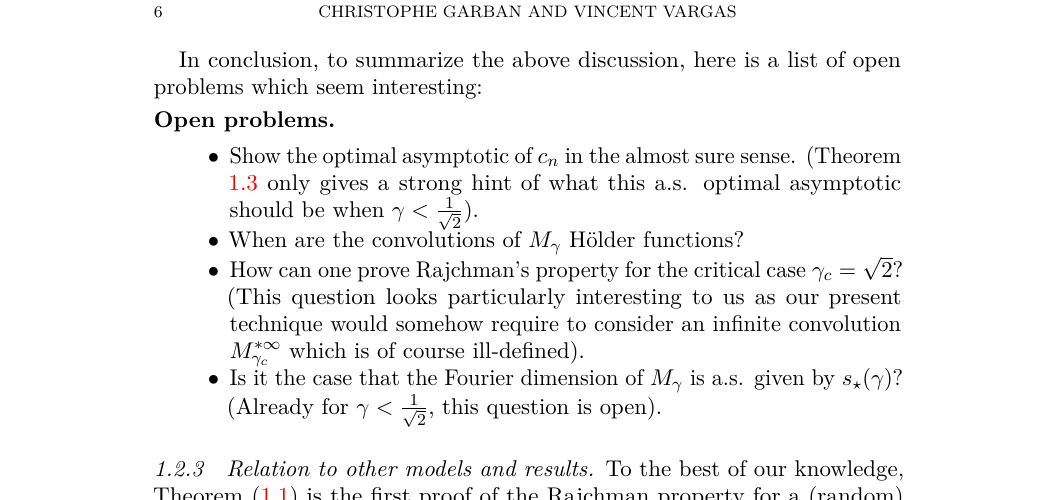
\includegraphics[width=\textwidth]{figures/open_problems_crop.png}
\end{center}

Lin, Qiu, and Tan subsequently proved the exact Fourier dimension predicted
in the source paper \cite{LinQiuTan}.  We show that this immediately gives an
explicit eventual-smoothing answer for every subcritical parameter.

\section*{Proof Intuition}

Convolution turns multiplication of Fourier coefficients into ordinary
powers.  If a measure has Fourier coefficients
$|\widehat\mu(n)|\lesssim |n|^{-s/2}$, then its $q$-fold convolution has
coefficients bounded by $|n|^{-qs/2}$.  Once
$qs/2>k+\alpha+1$, the Fourier series remains absolutely summable after
weighting by $|n|^{k+\alpha}$.  This gives a $C^{k,\alpha}$ density.  Taking
$s$ arbitrarily close to the exact Fourier dimension gives the claimed
threshold.

\section*{Deterministic Smoothing Lemma}

Write $m$ for normalized Haar measure on $\T=\mathbb R/(2\pi\mathbb Z)$ and
use
\[
                 \widehat\mu(n)=\int_\T e^{-in\theta}\,d\mu(\theta).
\]

\begin{proposition}\label{prop:deterministic}
Let $\mu$ be a finite Borel measure on $\T$.  Suppose that for some $s>0$,
\[
                  |\widehat\mu(n)|\leq C(1+|n|)^{-s/2}
                  \qquad(n\in\Z).
\]
Let $q\geq1$ and let $k\geq0$ be integers.  If $0<\alpha<1$ and
\[
                         k+\alpha<\frac{qs}{2}-1,
\]
then the $q$-fold convolution $\mu^{*q}$ has a $C^{k,\alpha}$ density with
respect to $m$.
\end{proposition}

\begin{proof}
The convolution identity gives
\[
                   \widehat{\mu^{*q}}(n)=\widehat\mu(n)^q.
\]
The assumed strict inequality implies
\[
 \sum_{n\in\Z}(1+|n|)^{k+\alpha}|\widehat\mu(n)|^q
 \leq C^q\sum_{n\in\Z}(1+|n|)^{k+\alpha-qs/2}<\infty.
\]
Consequently the Fourier series
\begin{equation}\label{eq:density}
                  f_q(\theta)=\sum_{n\in\Z}
                  \widehat\mu(n)^q e^{in\theta}
\end{equation}
converges absolutely and uniformly.  Its Fourier coefficients agree with
those of $\mu^{*q}$.  Since trigonometric polynomials are dense in $C(\T)$,
uniqueness of Fourier coefficients for finite measures gives
$d\mu^{*q}=f_q\,dm$.

The series obtained by differentiating \eqref{eq:density} $k$ times also
converges uniformly.  Moreover, using
$|e^{inh}-1|\leq 2|nh|^\alpha$, we have
\begin{align*}
 |f_q^{(k)}(\theta+h)-f_q^{(k)}(\theta)|
 &\leq 2|h|^\alpha
 \sum_{n\in\Z}|n|^{k+\alpha}|\widehat\mu(n)|^q.
\end{align*}
Thus $f_q^{(k)}$ is $\alpha$-H\"older, proving
$f_q\in C^{k,\alpha}(\T)$.
\end{proof}

\section*{Application to Gaussian Multiplicative Chaos}

For $0<\gamma<\sqrt2$, define
\begin{equation}\label{eq:Dgamma}
 D_\gamma=
 \begin{cases}
  1-\gamma^2,&0<\gamma<1/\sqrt2,\\
  (\sqrt2-\gamma)^2,&1/\sqrt2\leq\gamma<\sqrt2.
 \end{cases}
\end{equation}
This is the correlation-dimension threshold denoted $s_*(\gamma)$ in the
source paper.

\begin{theorem}\label{thm:main}
Let $M_\gamma$ be subcritical Gaussian multiplicative chaos on the circle.
Almost surely, simultaneously for every integer $q\geq1$, integer $k\geq0$,
and $0<\alpha<1$ satisfying
\begin{equation}\label{eq:threshold}
                       k+\alpha<\frac{qD_\gamma}{2}-1,
\end{equation}
the convolution $M_\gamma^{*q}$ has a $C^{k,\alpha}$ density.

In particular, if
\[
                   qD_\gamma>2,
\]
then $M_\gamma^{*q}$ has a H\"older-continuous density of every exponent
\[
                  0<\alpha<\frac{qD_\gamma}{2}-1.
\]
Thus a guaranteed first H\"older convolution power is
\[
                  q_0(\gamma)=\left\lfloor\frac{2}{D_\gamma}\right\rfloor+1.
\]
\end{theorem}

\begin{proof}
The exact Fourier-dimension theorem of \cite{LinQiuTan} states that, almost
surely,
\[
                         \dim_F(M_\gamma)=D_\gamma.
\]
By the definition of Fourier dimension, for every $s<D_\gamma$ there is an
almost surely finite random constant $C_s$ such that
\[
              |\widehat M_\gamma(n)|\leq
              C_s(1+|n|)^{-s/2}\qquad(n\in\Z).
\]
If \eqref{eq:threshold} holds, choose $s<D_\gamma$ sufficiently close to
$D_\gamma$ that $k+\alpha<qs/2-1$.  Proposition
\ref{prop:deterministic} then applies pathwise to $M_\gamma$.
\end{proof}

\begin{remark}[Scope]
The theorem proves eventual H\"older smoothing for every subcritical
$\gamma$ and gives all regularities forced by the known pointwise Fourier
decay.  It does not claim that the threshold $qD_\gamma>2$ is necessary.
Determining the first H\"older convolution power, including possible
endpoint behavior, remains open.
\end{remark}

\section*{Novelty Check}

Bounded searches through July 22, 2026 found the source question and the
later exact Fourier-dimension papers, but no statement of the convolution
corollary above.  The proof is elementary once exact Fourier decay is known;
novelty confidence is therefore moderate and should be checked by a
specialist in GMC harmonic analysis.

\begin{thebibliography}{9}

\bibitem{GarbanVargas}
C.~Garban and V.~Vargas,
\emph{Harmonic analysis of Gaussian multiplicative chaos on the circle},
arXiv:2311.04027 (2023).

\bibitem{LinQiuTan}
Z.~Lin, Y.~Qiu, and M.~Tan,
\emph{Harmonic analysis of multiplicative chaos, Part II: a unified approach
to Fourier dimensions}, arXiv:2505.03298 (2025).

\end{thebibliography}

\end{document}
